\section{Prelievo dei dati dal database}\label{sec:database}

Il database di \MonIQA{} è strutturato, per la parte che interessa per questo
progetto, come nel diagramma in Figura \vref{fig:dbarch}.

\begin{figure}[htb]
	\centering
	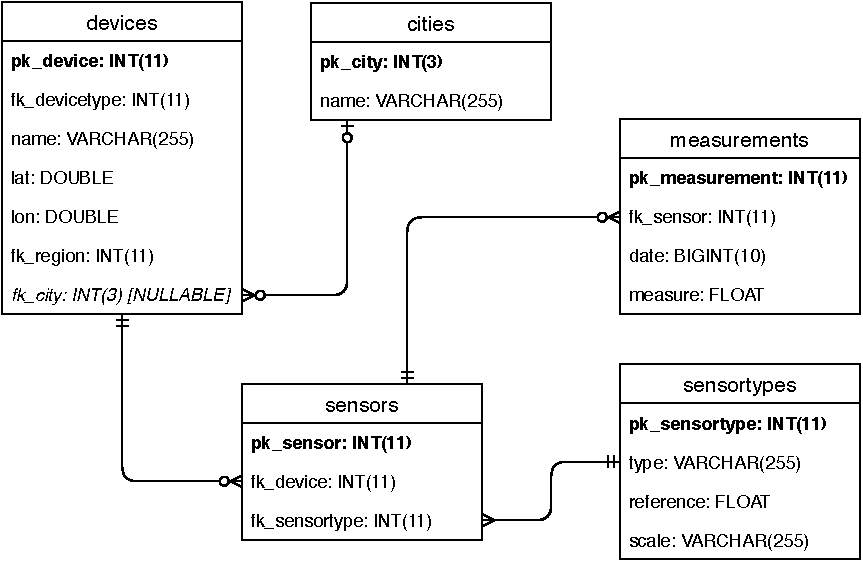
\includegraphics[width=\textwidth]{img/dbarch}
	\caption{Diagramma E-R del database di \MonIQA\@.}\label{fig:dbarch}
\end{figure}

La tabella \code{devices} contiene le stazioni di monitoraggio. Il campo
\code{fk\_city} è quello utilizzato per associare una provincia a ogni stazione,
come descritto nel paragrafo precedente. La tabella \code{cities} contiene
quindi le province.

La tabella \code{sensortypes} contiene un record per ogni tipo di sensore che
può essere installato sulle stazioni (i sensori si differenziano in base
all'inquinante che possono misurare) con il nome dell'inquinante che misurano, i
valori legali di riferimento e l'unità di misura per l'inquinante.

La tabella \code{measurements} contiene le misurazioni provenienti dai sensori
installate sulle stazioni, con il valore misurato e la data della misurazione.

Infine la tabella \code{sensors} mette in relazione le tabelle \code{devices},
\code{measurements} e \code{sensortypes} così da poter associare a ogni
misurazione la stazione e il sensore che l'ha effettuata.

Quindi, per prelevare i dati dal database, è stata sviluppata la query riportata
nel Listato \vref{lst:slowquery}.

\lstinputlisting[language=SQL, label={lst:slowquery}, caption={Query per il
prelievo dei dati dal database.}]{slow-query.sql}

In \code{\{\{PROVINCE\_NAME\}\}} andremo ad inserire il \emph{nome della
provincia} della quale si vogliono prelevare i dati; in
\code{\{\{START\_YEAR\}\}} e \code{\{\{END\_YEAR\}\}} inseriremo invece \emph{il
primo e l'ultimo anno del periodo di interesse}.

Divisioni e moltiplicazioni per \(1000\) sono necessarie in quanto, nel
database, tutte le date sono salvate come il numero di \emph{millisecondi}
trascorsi dalla mezzanotte del 01/01/1970, mentre le funzioni di MySQL
richiedono il numero di \emph{secondi} trascorsi da tale data.

La query ritorna quindi record aggregati per ogni anno, per ogni quarto di anno
e per ogni tipo di sensore \idest{inquinante}, fornendo la \emph{media delle
misurazioni di quel periodo per quell'inquinante} e \emph{il numero totale di
misurazioni} su cui la media è stata calcolata.
